\PageHeading{08}{案例A · 开学季小红书}{大学新生：从学习任务进入选机，而非从参数清单开始}
\ModeLocal
\begin{note}\small
\Lead{任务}\quad HUAWEI MateBook 14（鸿蒙版）／大学新生／开学季／对比选择／到店体验／小红书。\par
\Lead{实际结果}\quad 已确认大纲v1，6页1080$\times$1440 PNG；本轮实际运行规则策划、正文、初检与排版，未调用模型或ima。
\end{note}
\begin{center}
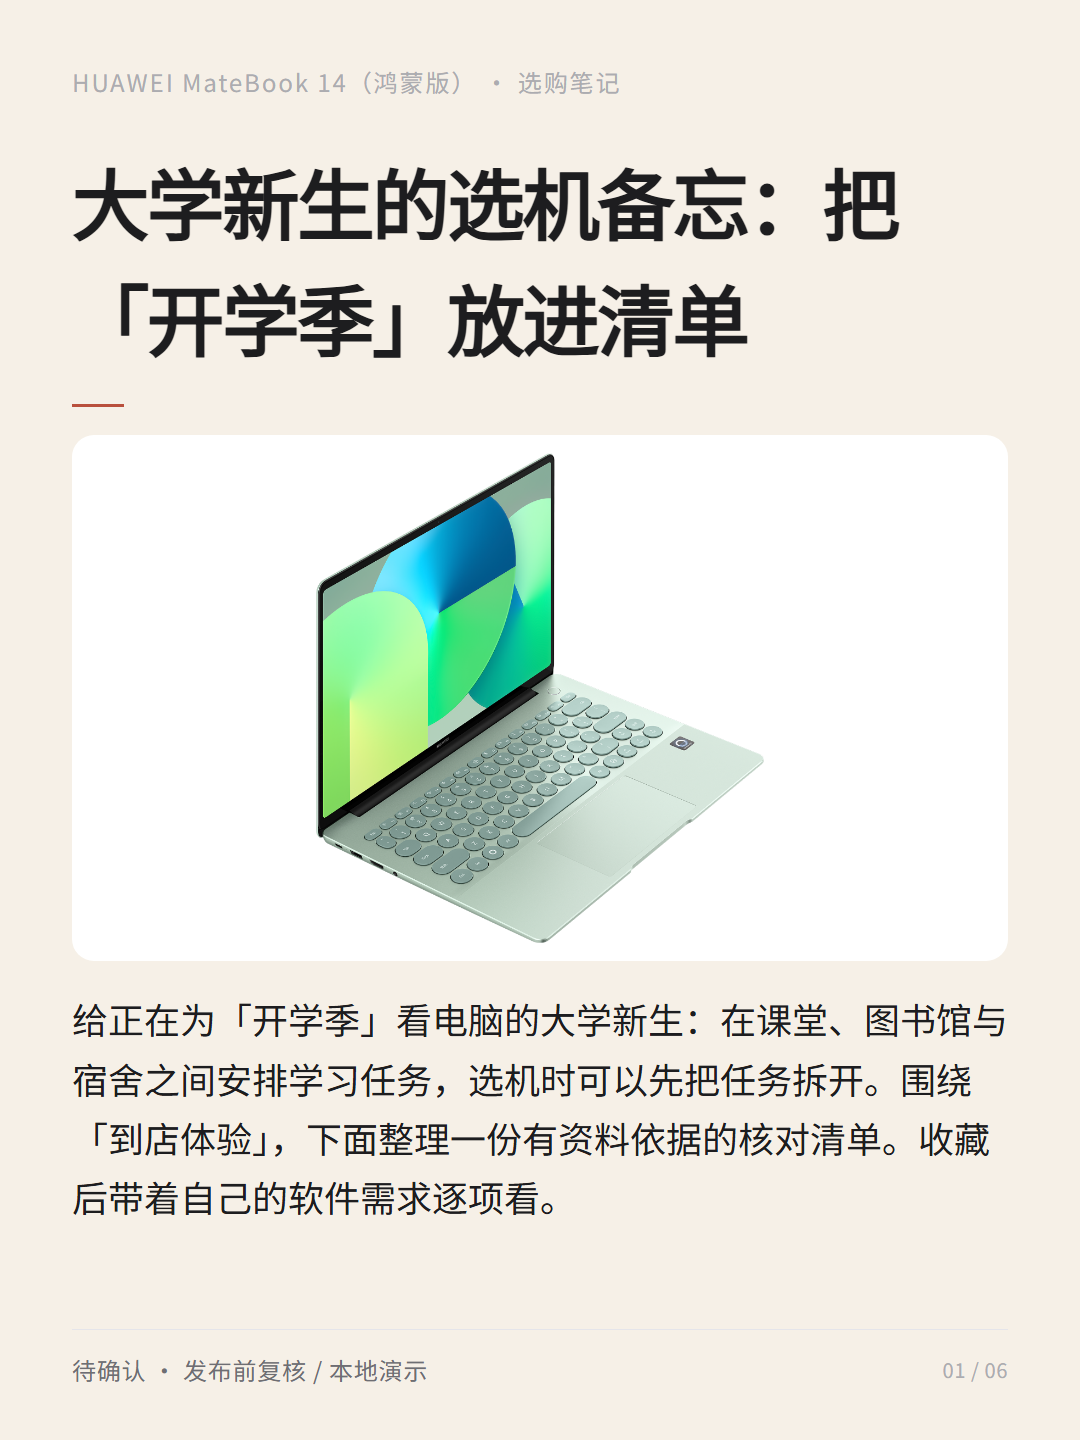
\includegraphics[width=.475\linewidth,height=101mm,keepaspectratio]{case-a-1.png}\hfill
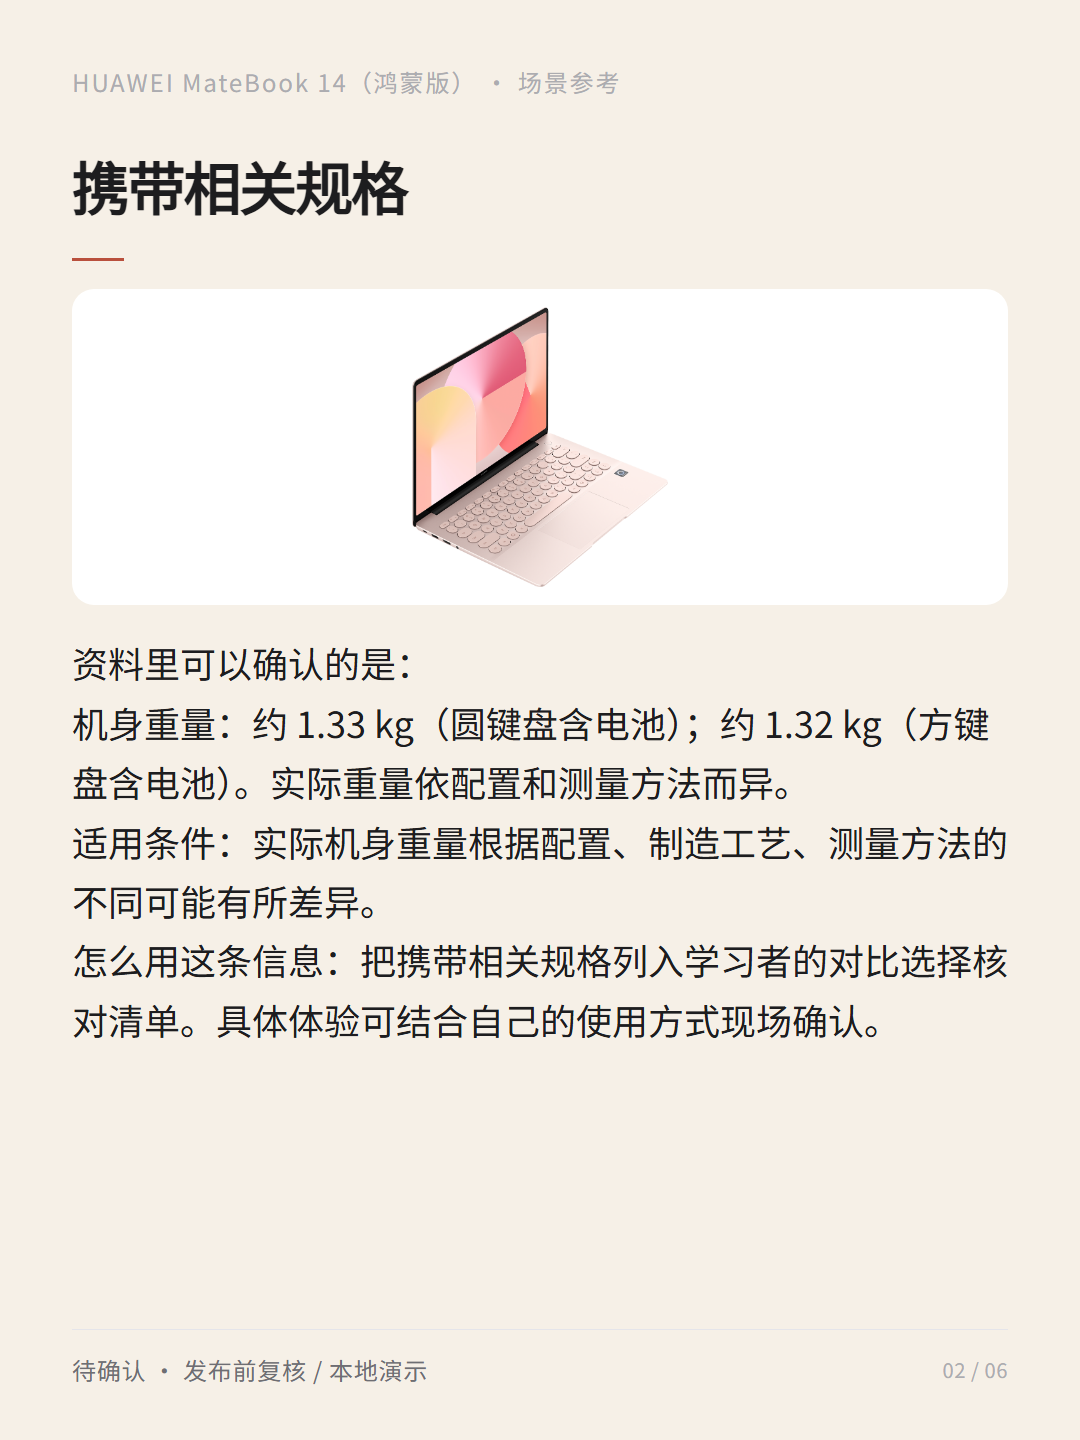
\includegraphics[width=.475\linewidth,height=101mm,keepaspectratio]{case-a-2.png}
\end{center}
\ImgCap{实际六页图文中的封面与第一内容页，保留“待确认／本地演示”页脚。原图保持产品形态与比例。}
\Sub{实际生成内容节选}
\begin{excerpt}\small
\Lead{\CaseATitle}\par
\CaseAIntro\par
\Lead{行动引导}\quad 把你常用的软件和使用场景留在评论区，一起补全选机清单。
\end{excerpt}
\Lead{策略解释}\quad 内容从课堂、图书馆与宿舍任务出发，优先组织携带、屏幕与电池维度，再提醒软件和版本核对。以收藏、清单和评论互动组织表达；没有伪造学生的亲测经历，也没有由电池容量推算续航时长。

\Lead{来源与核验}\quad 资料标题为“HUAWEI MateBook 14（鸿蒙版）·产品事实（本地资料）”及对应图片索引。段落事实与同型号原图随稿件保存。审核为needs\_attention，须核对当前销售版本及正式ima来源后再用于参赛验收。
\SourceNote{本轮实际生成，evidence/case-a.json；选录只作工程展示，不代表当前销售配置已核验。}
